
% ==============
%
% --------------
%-----
\section{Parallel Scaling of the EMG Model Using High Performance Computing}\label{sec:hpc_emg}
% in opendihu 2021 paper

After the parallel scaling of the multi-scale model has been investigated in moderately parallel scenarios with up to 27 processes in the previous sections, we now study the parallel scalability in High Performance Computing scenarios with larger degrees of parallelism.
We simulate the fiber based electrophysiology model consisting of a 0D subcellular model, the 1D electric conduction problem and the 3D bidomain equation, as described in \cref{sec:model_equations}.
We conduct these studies on the supercomputer Hawk at the High Performance Computing Center Stuttgart (HLRS). The system contains a total of 5632 compute nodes. Each compute node consists of two AMD EPYC 7742 processors with 64 cores each, a clock frequency of \SI{2.25}{\giga\hertz} and \SI{256}{\giga\byte} memory per node.

In the following, \cref{sec:weak_scaling_hawk} presents a weak scaling study, which scales the problem size up to a realistic number of \num{270000} muscle fibers in a biceps muscle.
Then, \cref{sec:mpi_rank_placement} shows measurements of the scaling behavior for the 1D model solver and gives details on MPI rank placement policies.

\subsection{Weak Scaling of the Fiber Based Electrophysiology Model}\label{sec:weak_scaling_hawk}

We simulate the fiber based electrophysiology model with EMG values on the muscle surface and the subcellular model of Hodgkin and Huxley \cite{Hodgkin1952}.
Corresponding simulation results of this scenario, also for the highly parallel runs, are presented in \cref{sec:effects_of_the_mesh_width_emg}.

In this weak scaling study, the number of fibers and number of processes is varied while their relation is kept approximately constant. The scenarios are constructed such that there are approximately 10 fibers per process, while maintaining a cube partitioning scheme in the 3D domain. The 0D subcellular and the 1D electric conduction problems on the fibers are solved with the \code{FastMonodomainSolver} class and the \code{`vc`} optimization type, which is the fastest available option in OpenDiHu. The Strang operator splitting scheme with Heun's method and the implicit Euler scheme are used. The 3D problem is solved using the conjugate gradient solver of PETSc and a relative tolerance on the residual norm of \num{1e-5}. 

The used timestep widths are $\dt_\text{0D}=\SI{1e-3}{\milli\second}$, $\dt_\text{1D}=\dt_\text{splitting}=\SI{2e-3}{\milli\second}$ and $\dt_\text{3D}=\SI{1}{\milli\second}$. Because only the scaling behavior is of interest in this study, the simulation end time is set to $t_\text{end}=\SI{2}{\milli\second}$.

% Hawk weak scaling
\begin{figure}[H]
  \centering%
  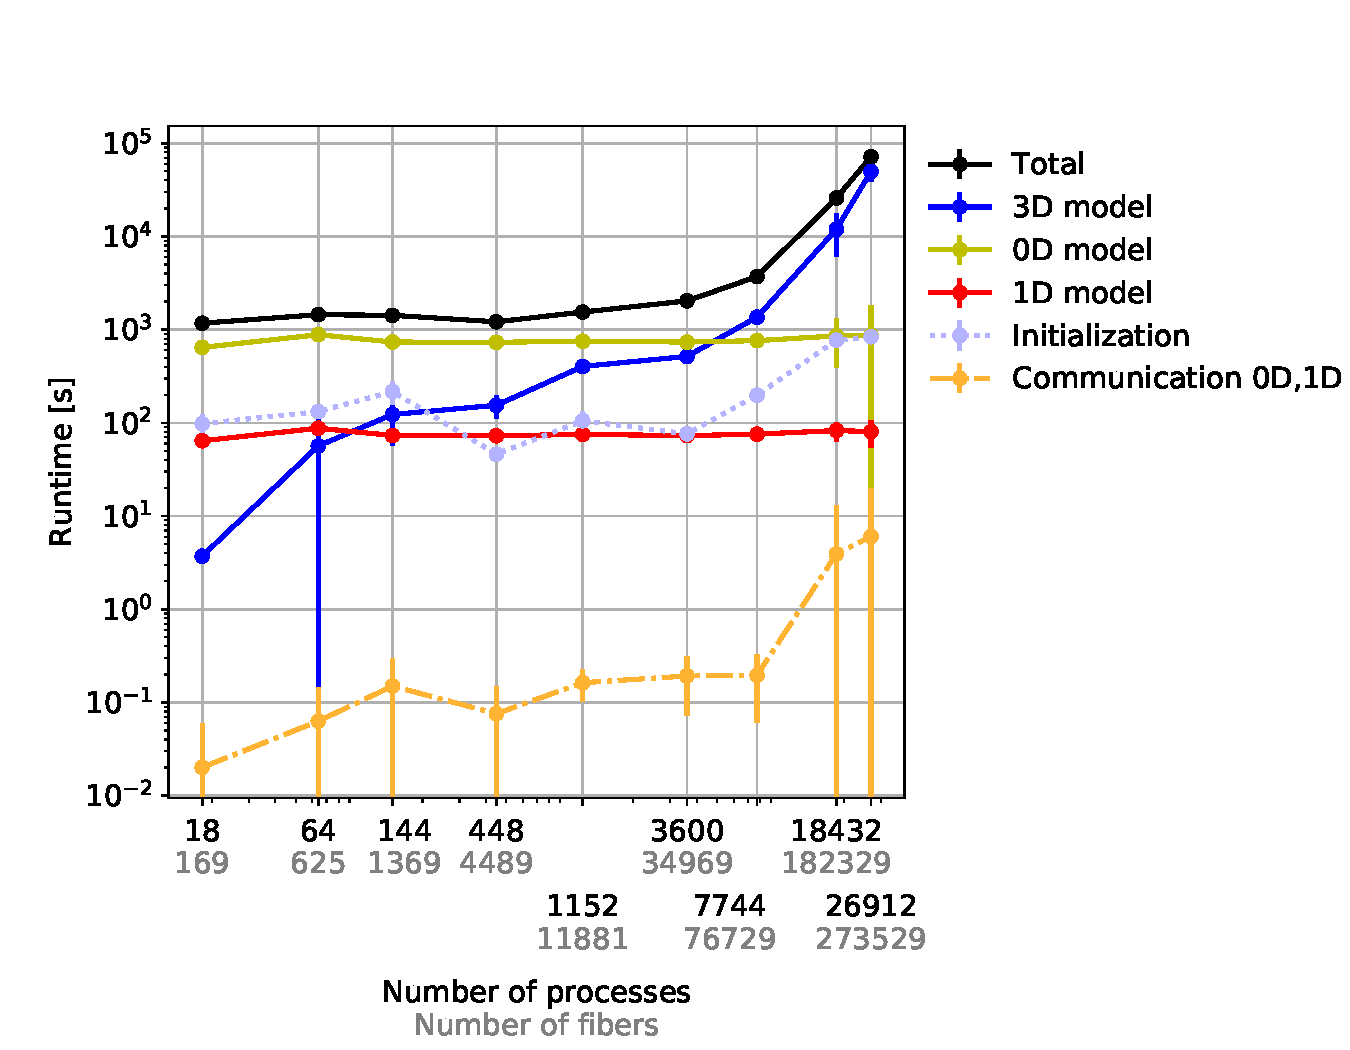
\includegraphics[width=\textwidth]{images/results/studies/hawk_weak_scaling.pdf}%
  \caption{Weak scaling of the fiber based electrophysiology model on the supercomputer Hawk simulating up to more than \num{270000} muscle fibers.}%
  \label{fig:hawk_weak_scaling}%
\end{figure}

\Cref{fig:hawk_weak_scaling} presents the resulting runtimes for the different parts of the simulation program: the solvers of the 0D, 1D and 3D models, the runtime for initialization and the runtime for the communication in the \code{FastMonodomainSolver}, as explained in \cref{sec:improved_parallel_solver_for_fiber_based}.
To relate the initialization runtime to the runtime of the solvers in a realistic scenario with longer simulation times, all runtimes except for the initialization are scaled to a simulation end time of $\SI{1}{\second}$.

The results show perfect weak scaling properties of the 0D and the 1D solver, given by the yellow and red lines. This is expected due to the construction of the algorithm and the parallel partitioning. The 0D problems are \say{embarrassingly parallel} and are solved independently of each other. In the 1D problem solver, the values are  transferred to a dedicated process, where the serial Thomas algorithm is employed for each fiber as a whole. Thus, the solution of all 1D problems is also performed independently of each other, but an additional communication step is required, before and after running the solver in each implicit time step of the 1D problem.
The plot shows a very small runtime for this communication even for higher parallelism, which is given by the orange dashed line.

The initialization of the computation involves parsing the Python script, which for the last data point requires \SI{35.1}{\s}, parallel file access and read operations of the mesh file, assembly of the 3D stiffness matrix and solution of the potential flow problem to obtain the fiber directions in the 3D mesh, which contains approximately \num{1e8} dofs for the last data point, code generation, compilation, linking and loading of the shared library for the subcellular problem, and initialization of all internal data structures.

Loading the mesh input file from the file system is the part of the initialization, which requires the most runtime.
The dotted light blue line in \cref{fig:hawk_weak_scaling} shows that the initialization time increases to a maximum value of \SI{839}{\s} for the largest problem size.

The runtime of the 3D model is shown by the blue line in \cref{fig:hawk_weak_scaling}. This part of the model is responsible for the highest portion of the total runtime starting from the scenario with \num{7744} fibers and \num{76729} processes. This increase is two-fold: first, the communication cost increases for a larger number of processes. Second, the number of iterations in the conjugate gradient solver increases for a larger number of unknowns.

\begin{table}
  \centering%
  \begin{tabular}{|r|r|r|r|r|r|r|r|r|}
    \hline
    \# processes  & 18 & 64  & 144 & 448  & 1152 & 3600 & 7744 & \num{26912}\\\hline
    \# iterations & 72 & 115 & 176 & 339  & 561  & 1056 & 1636 & 2807\\
    \hline
  \end{tabular}
  \caption{Scaling study of the fiber based muscle model: Number of iterations of the conjugate gradient solver for the 3D bidomain model in the weak scaling study presented in \cref{fig:hawk_weak_scaling}.}%
  \label{tab:cg_solver_iterations}%
\end{table}

In this weak scaling study, the number of conjugate gradient solver iterations increases from 72 for the first data point to \num{2807} for the last data point, as listed in \cref{tab:cg_solver_iterations}. The 3D problem of the last data point has \num{1e8} dofs. The exact numbers of dofs are also listed in \cref{tab:emg_study_parameters} in \cref{sec:effects_of_the_mesh_width_emg}.
Currently, the solution of the 3D problem uses no preconditioner. In future work, a multigrid solver could be employed for preconditioning, which could improve the weak scaling for large problem sizes.

In summary, the solution of the multi-scale model for fiber based electrophysiology without fat layer exhibits a very good weak scalability for up to \num{35000} fibers. For larger problem sizes, the solution of the 3D problem dominates and the weak scaling behavior deteriorates. However, the solution times are still feasible, as such large problems have been successfully solved in \cref{sec:effects_of_the_mesh_width_emg} of this work.


%         n_it
% nRanks      
% 18        72
% 64       115
% 144      176
% 448      339
% 1152     561
% 3600    1056
% 7744    1636
% 26912   2807

% partitioning  2* 2* 1=    4    7^2=    49 fibers, fibers/rank: 12.250000, need    1 nodes
% partitioning  3* 3* 2=   18   13^2=   169 fibers, fibers/rank: 9.388889, need    1 nodes
% partitioning  4* 4* 4=   64   25^2=   625 fibers, fibers/rank: 9.765625, need    1 nodes
% partitioning  6* 6* 4=  144   37^2=  1369 fibers, fibers/rank: 9.506944, need    3 nodes
% partitioning  7* 8* 8=  448   67^2=  4489 fibers, fibers/rank: 10.020089, need    7 nodes
% partitioning 12*12* 8= 1152  109^2= 11881 fibers, fibers/rank: 10.313368, need   18 nodes
% partitioning 15*15*16= 3600  187^2= 34969 fibers, fibers/rank: 9.713611, need   57 nodes
% partitioning 22*22*16= 7744  277^2= 76729 fibers, fibers/rank: 9.908187, need  121 nodes
% partitioning 24*24*32=18432  427^2=182329 fibers, fibers/rank: 9.891981, need  288 nodes
% partitioning 29*29*32=26912  523^2=273529 fibers, fibers/rank: 10.163830, need  421 nodes
% partitioning 40*40*32=51200  523^2=273529 fibers, fibers/rank: 5.342363, need  800 nodes
%                                           subdomains        user  total comp.        0D        1D   bidomain  duration_init  write       mem  n_it      n
% scenarioName                    nRanks                                                                                                                   
% hawk_weak_scaling_endtime_1.0_1 18         [3, 3, 2]  100.216111     2.346004  1.289333  0.128295   0.007430      97.870107    0.0  0.203 GB    72     18
%                                 64         [4, 4, 4]  134.937500     2.893596  1.765827  0.175330   0.113093     132.043904    0.0  0.315 GB   115     64
%                                 144        [6, 6, 4]  219.409583     2.850457  1.473133  0.146266   0.245577     216.559126    0.0  0.341 GB   176    144
%                                 448        [7, 8, 8]   48.533839     2.428730  1.463591  0.145278   0.308863      46.105109    0.0  0.584 GB   339    448
%                                 1152     [12, 12, 8]  295.241211     3.548350  1.489827  0.148680   1.321491     291.692861    0.0  0.385 GB   561   2304
%                                 3600    [15, 15, 16]   80.168103     4.069231  1.471832  0.146008   1.033123      76.098872    0.0  0.955 GB  1056   3600
%                                 7744    [22, 22, 16]  205.599181     7.422947  1.524253  0.151227   2.725283     198.176234    0.0  1.001 GB  1636   7744
%                                 18432   [24, 24, 32]  823.224210    51.681839  1.714082  0.165388  23.903565     771.542371    0.0  1.921 GB     0  18432
%                                 26912   [29, 29, 32]  982.392875   143.146126  1.739032  0.161190  99.627309     839.246749    0.0  2.066 GB  2807  26912

%-----
\subsection{Weak Scaling of the 1D Solver and MPI Rank Placement}\label{sec:mpi_rank_placement}


% performance/opendihu/08_0D1D_better_implementation
Next, we compare the different approaches to solve the 1D electric conduction part of the monodomain equation on the fibers in a High Performance Computing setting.
\Cref{fig:hazel_hen_rank_placement} shows a similar weak scaling study to the one in the last section with slightly different process counts. The study was carried out on the supercomputer Hazel Hen, a Cray XC30 system, which was installed until 2020 as the predecessor to Hawk at the High Performance Computing Center Stuttgart. The same problem as in the last section is solved, and, again, the relation between fibers and processes is 10:1. The partitionings were chosen in accordance with the compute nodes of Hazel Hen, which had 24 cores. The detailed problem sizes and partitionings can be found in \cite{Maier2019}.

\Cref{fig:hazel_hen_rank_placement} shows the runtimes of the same 0D and 1D solvers as in the last section by the solid yellow line for the 0D problem, the solid red line below for the 1D problem and the solid orange line for the communication. The perfect weak scaling for these parts is in line with the previous observations.

\begin{figure}
  \centering%
  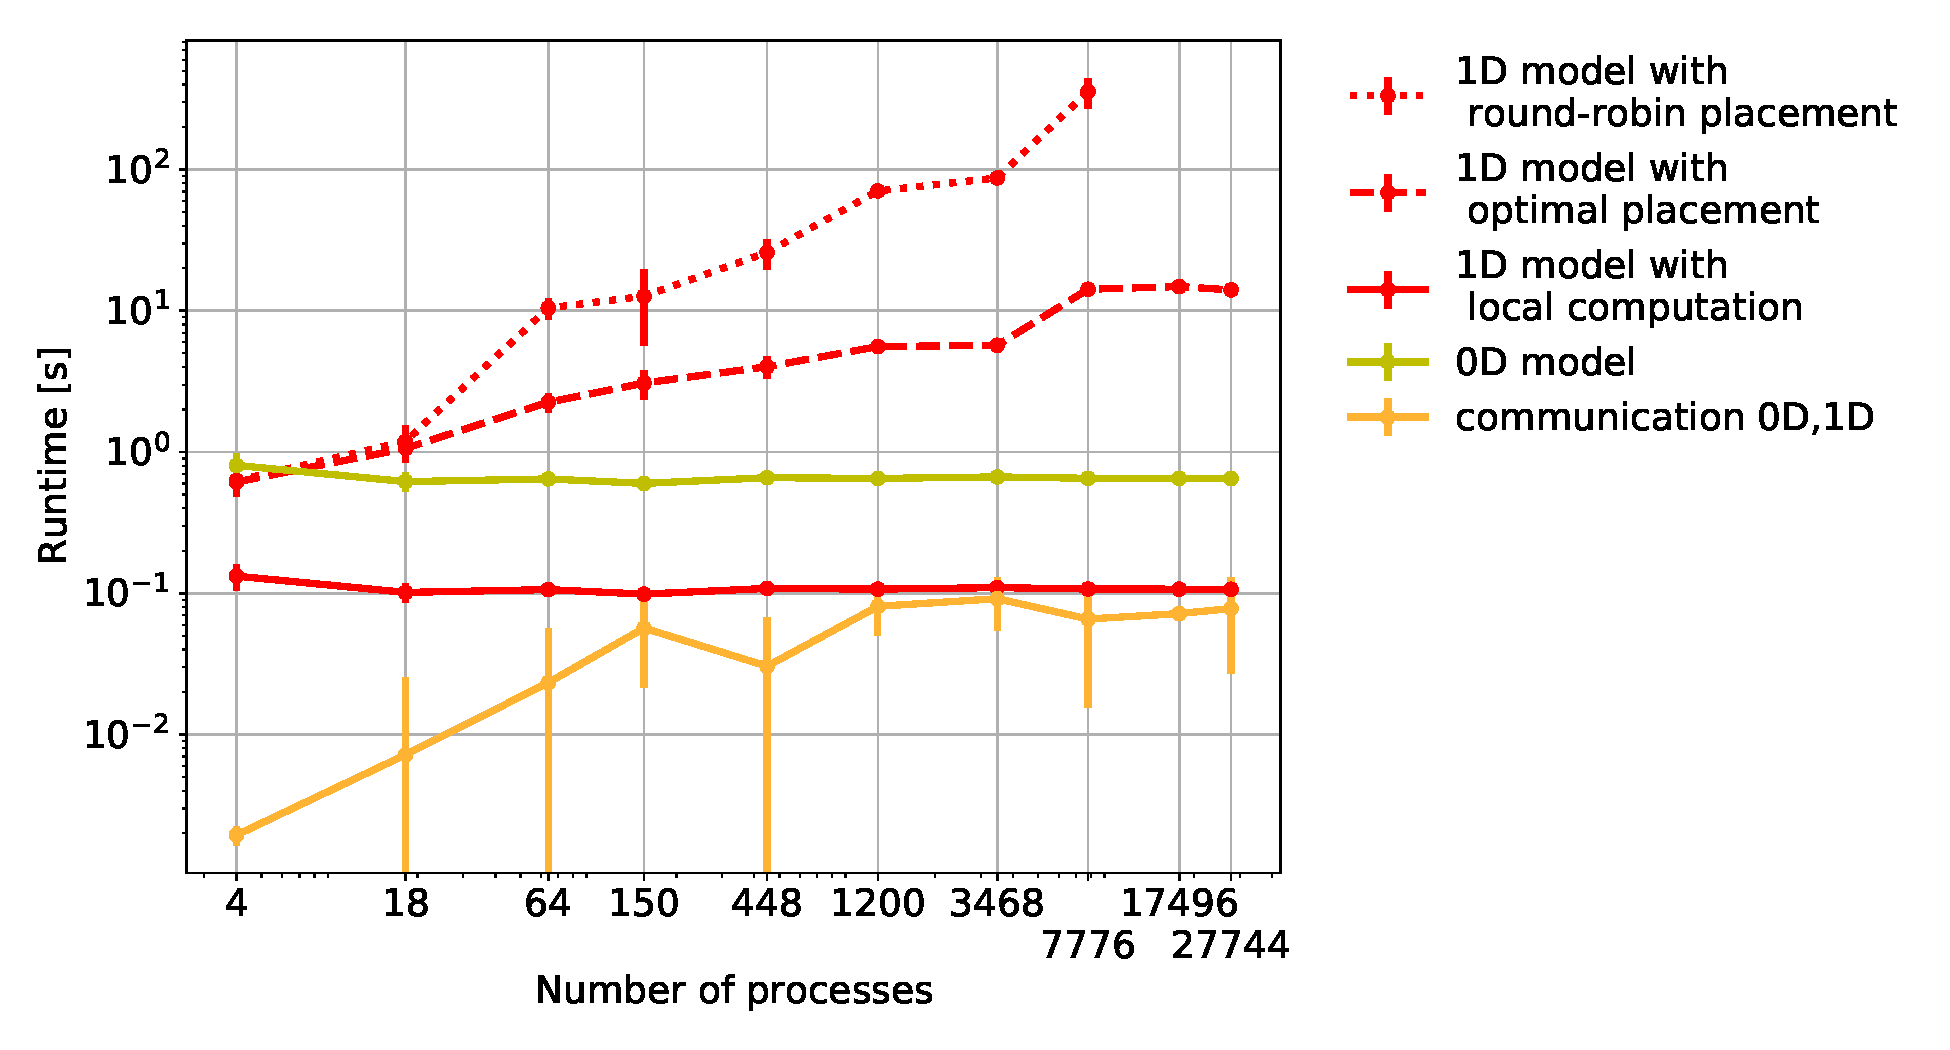
\includegraphics[width=\textwidth]{images/results/studies/Comparisonof0D-1Dcomputationschemes.pdf}%
  \caption{Scaling study of the fiber based muscle model: Weak scaling behavior of solvers for the 1D problem. Runtimes for the 1D solver with different rank placement strategy (dotted and dashed red lines) and the optimized runtimes of the \code{FastMonodomainSolver}, which combines the solution of the 0D and 1D problem (yellow and solid red lines, respectively).}% 
   \label{fig:hazel_hen_rank_placement}%
\end{figure}

In addition, we compare the weak scaling of the 1D solution, if a parallel conjugate gradient solver of PETSc is used for the problem on every fiber, instead of the serial Thomas algorithm. This setup corresponds to the \code{vc-aovs} scenario presented in \cref{sec:evaluation_of_code_gen}. As already noted earlier, the performance of this approach is worse. The dashed and dotted lines in \cref{fig:hazel_hen_rank_placement} present the runtimes of this approach for two different MPI rank placement strategies, but for the identical program. It can be seen that the runtimes increase with higher numbers of processes in both curves. This effect is the result of the 1D fiber problems being distributed to more processes, as the total number of processes increases. 

For example, in the scenarios with 1200 and 3468 processes, all fibers are distributed to 12 different processes. For the last three data points of the dashed curve, all fibers are distributed to 24 processes. As a result, the runtime to solve the 1D problems in the measurements with 1200 and 3468 processes is approximately equal, but lower than the runtime for the last three data points, where twice the amount of processors takes part in the solution of a single 1D problem.

The difference between the dotted and the dashed red curves is a different strategy to place the processes on the compute nodes. The dashed curve with the lower runtime corresponds to a placement of all fiber sharing processes on the same compute node. As the subdomain indices in the $n_x \times n_y \times n_z$ partitioning increase fastest in $x$-direction, then in $y$-direction and then in $z$-direction, and the fibers are aligned with the $z$ direction, the set of processes on a compute node contains MPI ranks that are offset with a constant stride of $n_x\,n_y$. This has to be ensured in the job scripts on the supercomputers by explicit MPI rank pinning.

If no such measures are taken, the default placement of MPI ranks on the compute nodes proceeds consecutively by filling the compute nodes in the order of the MPI ranks. This corresponds to a round-robin placement of the fibers on the compute nodes, which is the worst possible way of distributing MPI ranks to compute nodes. All processes that compute a fiber are potentially located on different nodes and have to communicate over compute node boundaries.
\Cref{fig:hazel_hen_rank_placement} shows the resulting runtimes by the upper, dotted red curve. The difference in runtime increases to one order of magnitude for the highest number of cores.

Thus, it is important to properly handle MPI rank placement on compute clusters with multiple compute nodes. As a consequence, we also configured rank placement on the supercomputer Hawk accordingly in all our studies on this system.

% ------------
%
% f===========


\section{Performance Studies of the Solid Mechanics Solver}\label{sec:performance_solid_mechanics}

%(BM TODO read)

Next, we address the performance of the solid mechanics solver. 
Its runtime in OpenDiHu is given by the call to the nonlinear solver of PETSc. PETSc, in turn, calls two functions in OpenDiHu, which evaluate the nonlinear function to be solved and the Jacobian of the nonlinear function for a given vector of unknowns.
In the following, \cref{sec:analytic_numeric_jacobian} compares an analytic and a numerical computation scheme for the Jacobian, and \cref{sec:vectorization_analytic_jacobian} studies the impact of vectorization in this computation.

\subsection{Analytic and Numerical Computations of the Jacobian}\label{sec:analytic_numeric_jacobian}

The computation of the Jacobian can be done in two ways. The first possibility is done by PETSc, which uses finite differences to numerically estimate the value of the Jacobian. The second possibility is to evaluate the respective analytic formulation within OpenDiHu. This analytic formulation is derived in \cref{sec:discretization_mechanics} and uses the SEMT library \cite{semt} to differentiate the mechanics model given by a strain energy function at compile time.

\begin{figure}
  \centering%
  %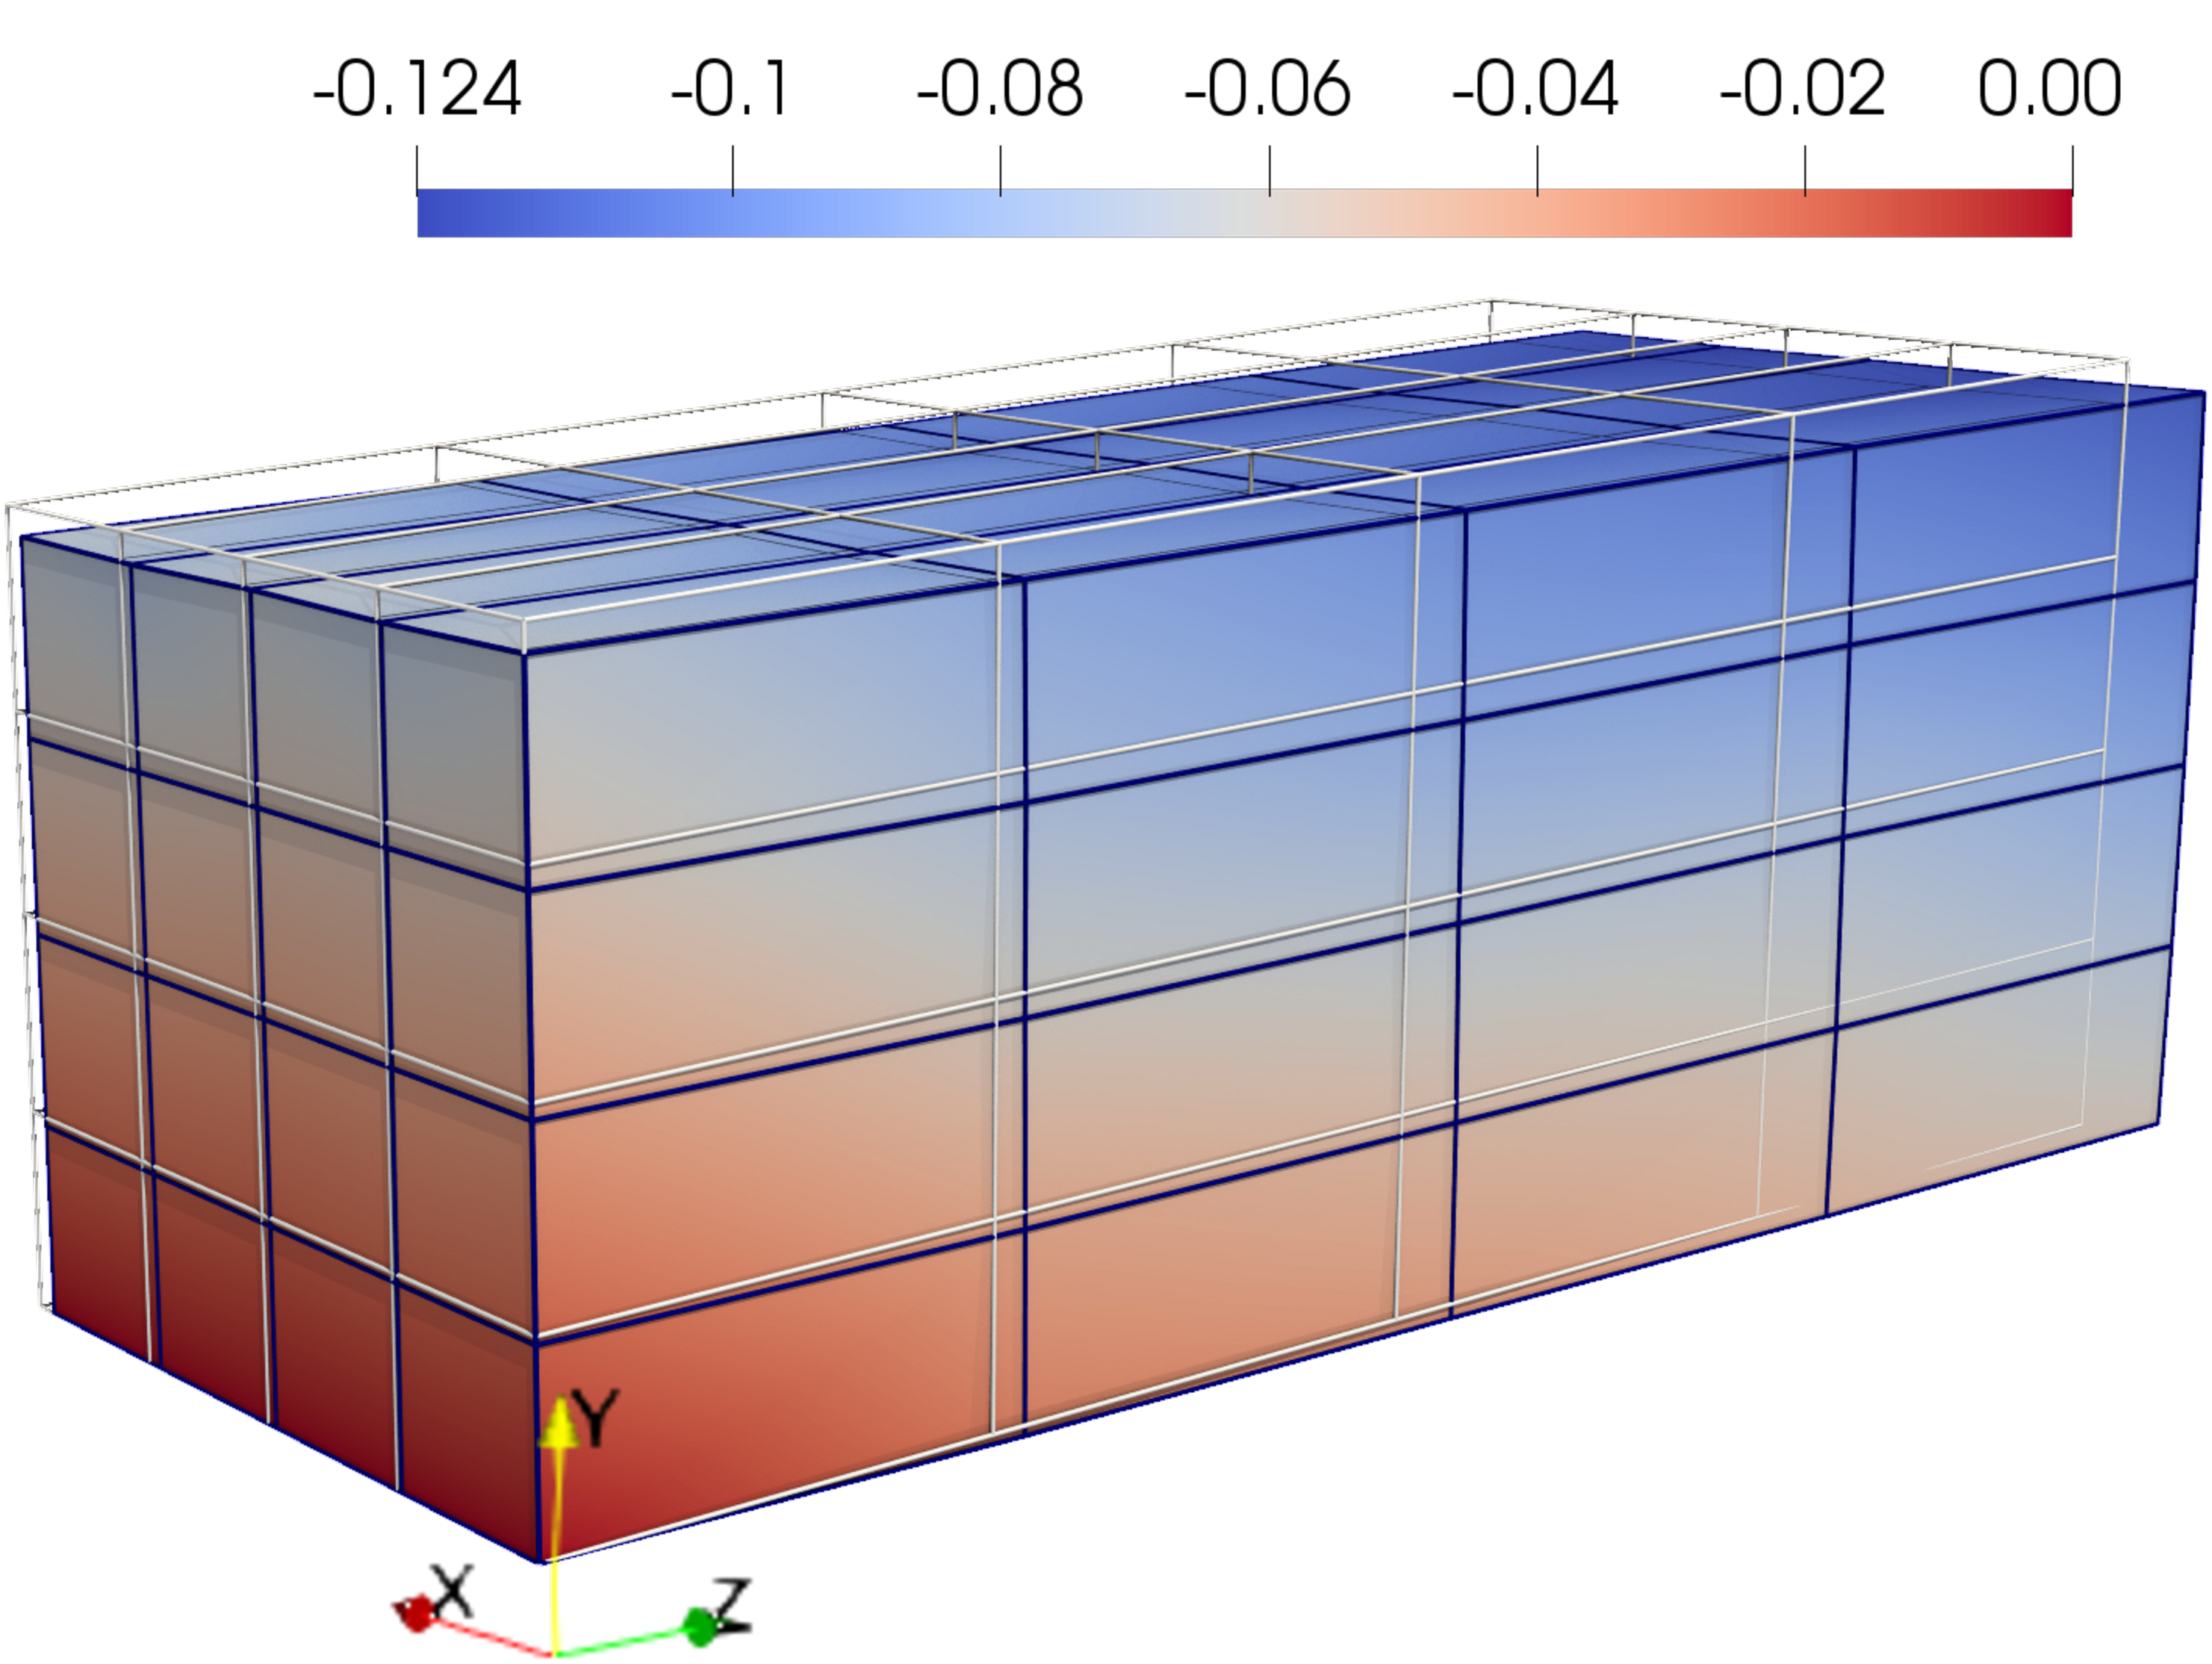
\includegraphics[width=0.4\textwidth]{images/results/studies/mechanic_scenario.png}%
  \def\svgwidth{0.6\textwidth}
  \input{images/results/studies/mechanic_scenario.pdf_tex}%
  \caption{Scaling study for solid mechanics: Visualization of the solid mechanics problem used in the weak scaling studies. The box is extended by a surface load at the right end. The wireframe shows the reference configuration, the colored mesh shows the current configuration where the color corresponds to the displacements $u_y$ in vertical direction.}%
  \label{fig:mechanic_scenario}%
\end{figure}

To compare both approaches, we simulate a tension test, where a cuboid domain is extended by an applied force. 
The box is shown in \cref{fig:mechanic_scenario} and has physical dimensions $\SI{2}{\cm} \times \SI{2}{\cm} \times \SI{5}{\cm}$. The left face of the box is fixed at $z=0$ and the two edges of the left face at $x=0$ and $y=0$ are also fixed to prevent rotation of the body. On the right face, a constant surface load with a total force of $10$ is applied.
The material model is the incompressible transversely isotropic Mooney-Rivlin description given in \cref{eq:transiso_mooney_rivlin}, which is also used for the muscle tissue. However, no active stress is considered. The material parameters are chosen as $c_1=2, c_2=3, b = 4$ and $d = 5$. The fiber direction lies in the $y-z$ plane and has an angle of $\SI{40}{\degree}$ to the $z$ axis.
As a result, the box slightly bends in negative $y$ direction, as can be seen in \cref{fig:mechanic_scenario}. In this figure, the volume of the deformed object is colored according to the displacement in $y$ direction.

We solve the problem using the Newton solver of PETSc with a secant line search over the $L_2$ norm of the function. The absolute and relative residual tolerances are set to \SI{1e-5}, which leads to approximately 5 Newton iterations. The parallel direct solver of the MUMPS package \cite{Mumps2017} is used to solve the linear system in every Newton iteration.

We compare the runtimes of numerically and analytically computing the Jacobian in this problem. We vary the number of processes and the problem size in a weak scaling setting, such that there are exactly 8 3D elements per process. A dual-socket AMD EPYC 7742 64-core processor with clock speed of \SI{2.25}{\giga\hertz}, a total core count of 128 and \SI{1.96}{\tera\byte} RAM is used. We vary the number of processes between one and 256 processes. For more than 128 processes, hyperthreading is used.

\Cref{fig:numeric_analytic} shows the runtimes to solve the nonlinear system by the orange and purple lines in a double logarithmic plot. An increasing runtime for higher process counts is observed for both computation approaches. The curves have a higher slope for more than 128 processes, when the computation uses more processes than physical cores in the processor.

The computation of the Jacobian requires $\O(n)$ non-zero entries to be calculated as the matrix has a banded sparsity structure, where $n$ is the number of degrees of freedom or elements in the 3D mesh. The number of non-zero Jacobian entries is, thus, constant in the weak scaling setup.
However, \cref{fig:numeric_analytic} shows a linearly increasing runtime for the numerical computation of the Jacobian, which can be seen by the comparison with the plotted linear function. 
The finite difference scheme of PETSc has no information about the sparsity pattern and estimates all $\O(n^2)$ matrix entries.

The runtimes for the analytic computation are only slightly increasing in the weak scaling, which is as expected. This approach only computes the non-zero entries of the Jacobian. Moreover, the values of the material elasticity tensor $\C$ can be computed once and reused for every entry of the Jacobian.

The comparison between the approaches shows lower computation times for the analytic approach by factors between \num{6.2} for one process and \num{450} for 192 processes. 
In conclusion, the analytic formula for the Jacobian, which is implemented in OpenDiHu, allows us to speed up the mechanics computations and to compute larger problem sizes in feasible runtimes.
%[2, 3, 4, 5],  # c1, c2, b1, d1

%performance/opendihu/22_solid_mechanics_vectorization
\begin{figure}
  \centering%
  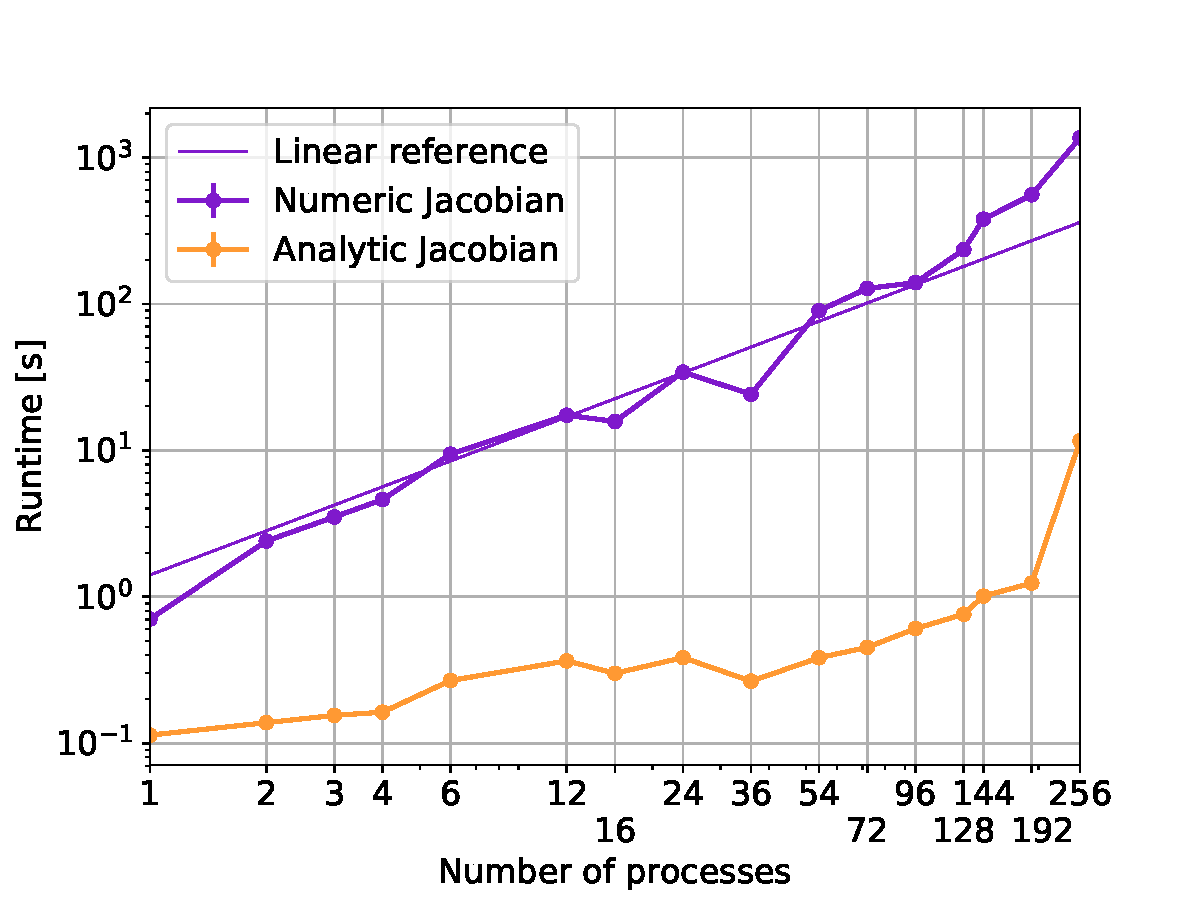
\includegraphics[width=0.7\textwidth]{images/results/studies/numeric_analytic.pdf}%
  \caption{Weak scaling of the nonlinear mechanics solver. The runtime to solve the nonlinear system equation is given for the numerical and for the analytic computation approaches for the Jacobian matrix.}%
  \label{fig:numeric_analytic}%
\end{figure}
                            %user duration_init  write     nonlin       mem    n
%scenarioName   nRanks                                                          
%not_vectorized 1        1.790000             0    0.0   1.242300  0.096 GB    1
               %2        2.255000             0    0.0   1.685440  0.128 GB    2
               %3        2.190000             0    0.0   1.574477  0.129 GB    3
               %4        2.295000             0    0.0   1.660710  0.129 GB    4
               %6        2.830000             0    0.0   2.152498  0.133 GB    6
               %12       3.502500             0    0.0   2.658058  0.156 GB   12
               %16       4.000000             0    0.0   3.130890  0.162 GB   16
               %24       4.463750             0    0.0   3.586197  0.165 GB   24
               %36       5.309167             0    0.0   4.027296  0.160 GB   36
               %54       6.746852             0    0.0   5.433671  0.175 GB   54
               %96      12.793854             0    0.0   9.704076  0.255 GB   96
               %128     17.626562             0    0.0  13.354177  0.279 GB  128
               %144     22.389931             0    0.0  17.560908  0.295 GB  144
               %192     28.981458             0    0.0  22.698083  0.336 GB  192
               %256     38.794062             0    0.0  29.661437  0.403 GB  256
%vectorized     1        1.200000             0    0.0   0.774613  0.100 GB    1
               %2        1.620000             0    0.0   1.197025  0.134 GB    2
               %3        1.536667             0    0.0   1.083777  0.134 GB    3
               %4        1.632500             0    0.0   1.175385  0.134 GB    4
               %6        2.130000             0    0.0   1.612840  0.139 GB    6
               %12       2.848333             0    0.0   2.151758  0.161 GB   12
               %16       3.383125             0    0.0   2.691964  0.167 GB   16
               %24       3.762083             0    0.0   3.028075  0.169 GB   24
               %36       4.418889             0    0.0   3.323164  0.165 GB   36
               %54       6.148889             0    0.0   5.048258  0.179 GB   54
               %96      12.345937             0    0.0   9.352379  0.260 GB   96
               %128     16.575547             0    0.0  12.661745  0.285 GB  128
               %144     20.970833             0    0.0  16.276117  0.299 GB  144
               %192     27.397344             0    0.0  21.641200  0.345 GB  192
               %256     38.021875             0    0.0  29.648075  0.414 GB  256


\subsection{Vectorization of the Analytic Jacobian Computations}\label{sec:vectorization_analytic_jacobian}

In the assembly of finite element system matrices of any kind, contributions are computed on an element level and then combined to form a global system matrix. In OpenDiHu, this algorithm can be vectorized by performing analog but independent computations for multiple elements concurrently in multiple SIMD lanes. This vectorization uses the \emph{Vc} library, similar to the optimizations of the subcellular model solver presented in \cref{sec:performance_studies_of_the_e}. As this vectorization significantly increases compilation times, the feature is turned off by default and has to be enabled before compilation.

In this section, we evaluate the effect of vectorized system matrix computations for the Jacobian matrix of the nonlinear solid mechanics solver. We conduct a similar weak scaling study as before using the same scenario, but an eight times larger number of elements for each measurement. We compare the runtime to solve the nonlinear problem using analytic Jacobian computations with disabled and enabled vectorization.

\begin{figure}
  \centering%
  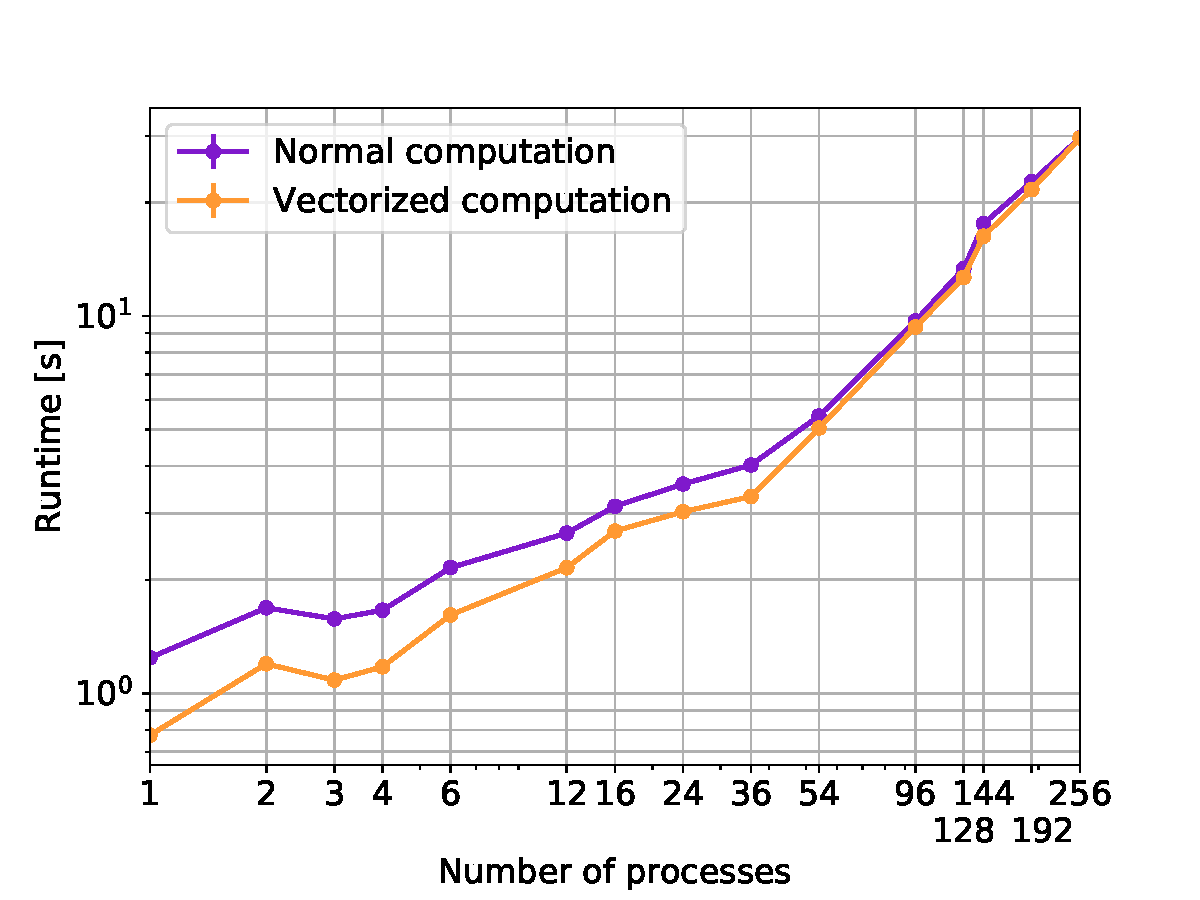
\includegraphics[width=0.8\textwidth]{images/results/studies/vectorized.pdf}%
  \caption{Scaling Study for the solid mechanics solver: Weak scaling study to evaluate vectorization in the computation of the Jacobian.}%
  \label{fig:vectorized_jacobian}%
\end{figure}

\Cref{fig:vectorized_jacobian} presents the resulting runtimes for the entire nonlinear solver. 
The vectorized computation shows speedups from \num{1.6} for one process to \num{1.06} for 128 processes. The theoretically possible speedup is four, as the processor supports the AVX2 instruction set with a vector register length of four double-precision values. The measured speedups are lower, because the computation of the Jacobian is only one portion of the computations in the nonlinear solver. 
%For some operations during the computation of the Jacobian, the individual values have to be unpacked from the vector registers, e.g., for the check if the jacobian

In summary, the vectorized computation of Jacobian matrices can reduce runtimes for the nonlinear solver. A runtime reduction of \SI{38}{\percent} (corresponding to the speedup of \num{1.6}) was observed for the serial scenario. The performance gain is largest for small problem sizes and small numbers of processes, and gets less prominent for larger degrees of parallelism.
                            %user duration_init  write     nonlin       mem    n
%scenarioName   nRanks                                                          
%not_vectorized 1        1.830000             0    0.0   1.254970  0.095 GB    1
               %2        2.295000             0    0.0   1.690225  0.127 GB    2
               %3        2.170000             0    0.0   1.565473  0.130 GB    3
               %4        2.275000             0    0.0   1.664090  0.130 GB    4
               %6        2.838333             0    0.0   2.155187  0.134 GB    6
               %12       3.481667             0    0.0   2.625879  0.156 GB   12
               %16       3.996250             0    0.0   3.150559  0.162 GB   16
               %24       4.477917             0    0.0   3.582378  0.164 GB   24
               %36       6.520278             0    0.0   3.237879  0.140 GB   36
               %54       6.417222             0    0.0   3.185654  0.140 GB   54
               %96      11.051667             0    0.0   9.128967  0.210 GB   96
               %128     14.289687             0    0.0  11.515929  0.230 GB  128
               %144     18.201042             0    0.0  10.828896  0.215 GB  288
               %192     22.485521             0    0.0  13.421127  0.257 GB  192
               %256     27.934727             0    0.0  17.611625  0.336 GB  256
%vectorized     1        1.210000             0    0.0   0.769704  0.101 GB    1
               %2        1.615000             0    0.0   1.192770  0.133 GB    2
               %3        1.533333             0    0.0   1.088080  0.134 GB    3
               %4        1.630000             0    0.0   1.172938  0.134 GB    4
               %6        2.153333             0    0.0   1.618572  0.139 GB    6
               %12       2.712500             0    0.0   2.095109  0.161 GB   12
               %16       3.403125             0    0.0   2.707476  0.168 GB   16
               %24       3.792500             0    0.0   3.024117  0.168 GB   24
               %36       5.683056             0    0.0   2.602400  0.145 GB   36
               %54       5.753148             0    0.0   2.663889  0.145 GB   54
               %96      10.421667             0    0.0   8.659787  0.215 GB   96
               %128     13.699063             0    0.0  11.105826  0.236 GB  128
               %144     16.196667             0    0.0   9.629186  0.220 GB  288
               %192     20.471302             0    0.0  12.320687  0.264 GB  192
               %256     26.646992             0    0.0  17.193776  0.345 GB  256

\begin{reproduce_no_break}
  The scripts to run the studies in this scenario and to create the plots of \cref{fig:numeric_analytic,fig:vectorized_jacobian} are available in the repository at \href{https://github.com/dihu-stuttgart/performance}{github.com/dihu-stuttgart/performance}
  in the directory \code{opendihu/22_solid_mechanics_vectorization}.
\end{reproduce_no_break}
% --------------------t
%
% ======================

% numerical investigations
\section{Numerical Studies}\label{sec:numerical_studies}

Next, we perform numerical studies to evaluate mesh resolutions and linear solvers. 
\Cref{sec:action_potential_velocity} addresses the mesh width of the 1D problem. \Cref{sec:multidomain_solvers} evaluates different numerical solver choices for the multidomain model.
\subsection{Effect of the Mesh Width on the Action Potential Propagation Velocity}\label{sec:action_potential_velocity}

The numerical parameters of a simulation scenario such as mesh widths and timestep widths should be chosen, such that the resulting numerical errors are balanced between all model components. In the simulation of activated muscle fibers, the propagation velocity of the action potentials is an important quantity, which also influences the macroscopic outcome of the EMG recordings. Thus, we investigate the effect of numerical parameters on the propagation velocity.

%performance/opendihu/02_propagation_velocity
\begin{figure}%
  \centering%
  \begin{subfigure}[t]{0.45\textwidth}%
    \centering%
    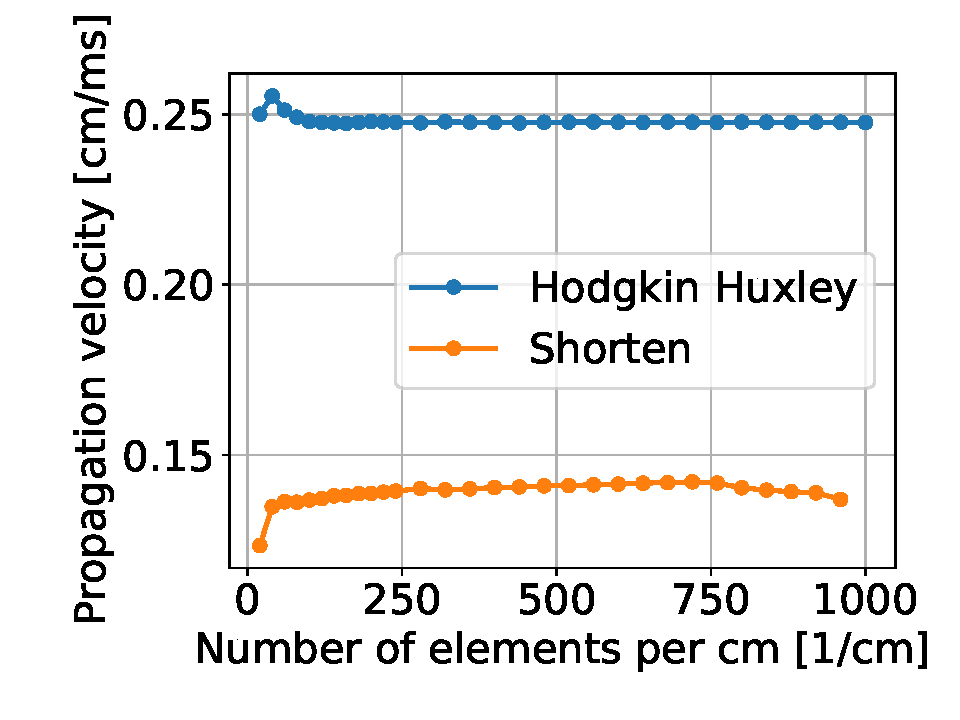
\includegraphics[width=\textwidth]{images/results/studies/propagation_velocity.pdf}%
    \caption{Propagation velocities over spatial resolution of the 1D mesh.}%
    \label{fig:propagation_velocity_comparison}%
  \end{subfigure}
  \,
  \begin{subfigure}[t]{0.45\textwidth}%
    \centering%
    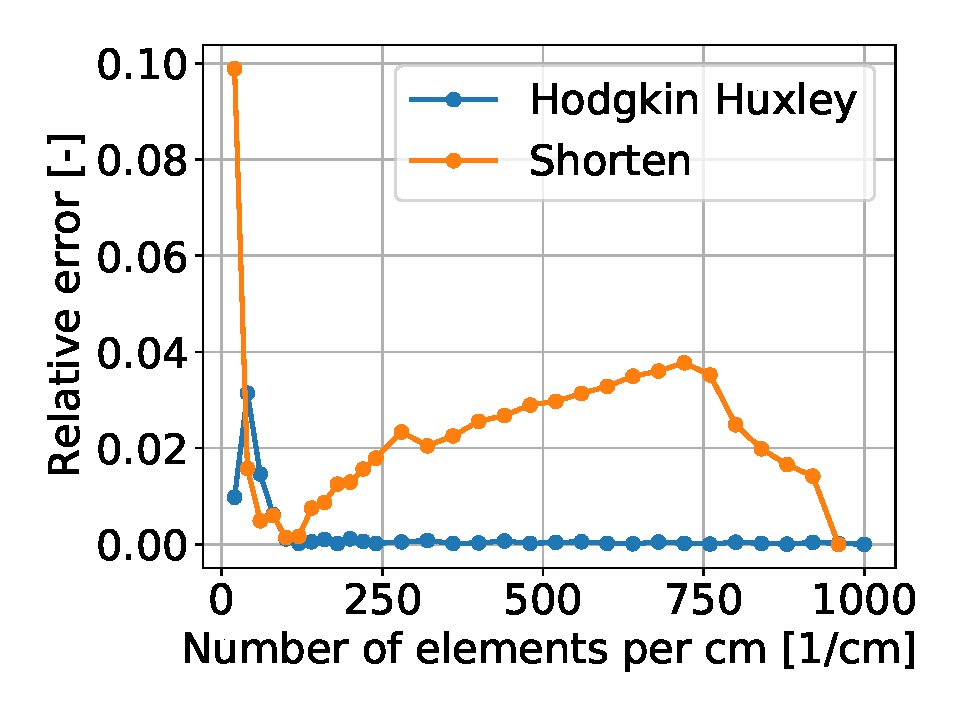
\includegraphics[width=\textwidth]{images/results/studies/propagation_velocity_rel_error.pdf}%
    \caption{Relative error of the propagation velocities over spatial resolution of the 1D mesh.}%
    \label{fig:propagation_velocity_rel_error}%
  \end{subfigure}   
  \caption{Influence of the mesh width on the propagation velocity of the action potential for the subcellular models of Shorten and Hodgkin-Huxley in the fiber-based electrophysiology simulation. This study is used to determine the 1D mesh width.}%
  \label{fig:propagation_velocity}%
\end{figure}%

In the first study, we consider a single fiber given by a 1D mesh, where the monodomain equation \cref{eq:monodomain} is used.
We measure the error of the propagation velocity depending on the mesh width. A fiber with a physical length of \SI{4}{\cm} is used and discretized by different numbers of 1D elements. We stimulate the fiber at its center at the beginning of the simulation and run the simulation until an end time of \SI{28}{\ms}. An action potential propagates along the fiber. We determine the location of the propagating peak at the end and compute the propagation velocity.

\Cref{fig:propagation_velocity_comparison} shows the resulting values of the propagation velocity for the Hodgkin-Huxley and Shorten subcellular models for varying mesh resolutions. It can be seen that the velocities level out at a constant value for finer mesh discretizations. The absolute value of the propagation velocity is different for the two subcellular models and depends on various model parameters.

For a quantitative evaluation, we examine the error of the propagation velocity, which is estimated by comparing each run with the value from the finest simulation. 
One issue with comparing propagation velocities on discretized meshes is that the measured velocity can only be calculated as number of elements traversed per time interval. Thus, the measurements for different mesh resolutions have different accuracies, not only due to the usual discretization error in the finite element approach. This issue can be reduced if a long enough time is simulated, such that the action potential propagates a large enough distance in terms of multiples of the element width.

\Cref{fig:propagation_velocity_rel_error} shows the resulting relative error of the propagation velocity. It can be seen that, for the Hodgkin Huxley model, the error gets close to zero for 100 elements per centimeter of fiber length. For the Shorten model, this mesh resolution also exhibits a low relative error. However, the error increases again for higher mesh resolutions before decreasing again starting at approximately 750 elements per centimeter. 

As a result, we use a 1D mesh resolution of 100 elements per centimeter for all muscle fibers in all our simulations. For a biceps muscle of \SI{14.8}{\cm} length, this leads to muscle fiber discretizations with 1480 elements and 1481 nodes.

%performance/opendihu/03_dx_dt_dependence
%\begin{figure}
%  \centering%
%  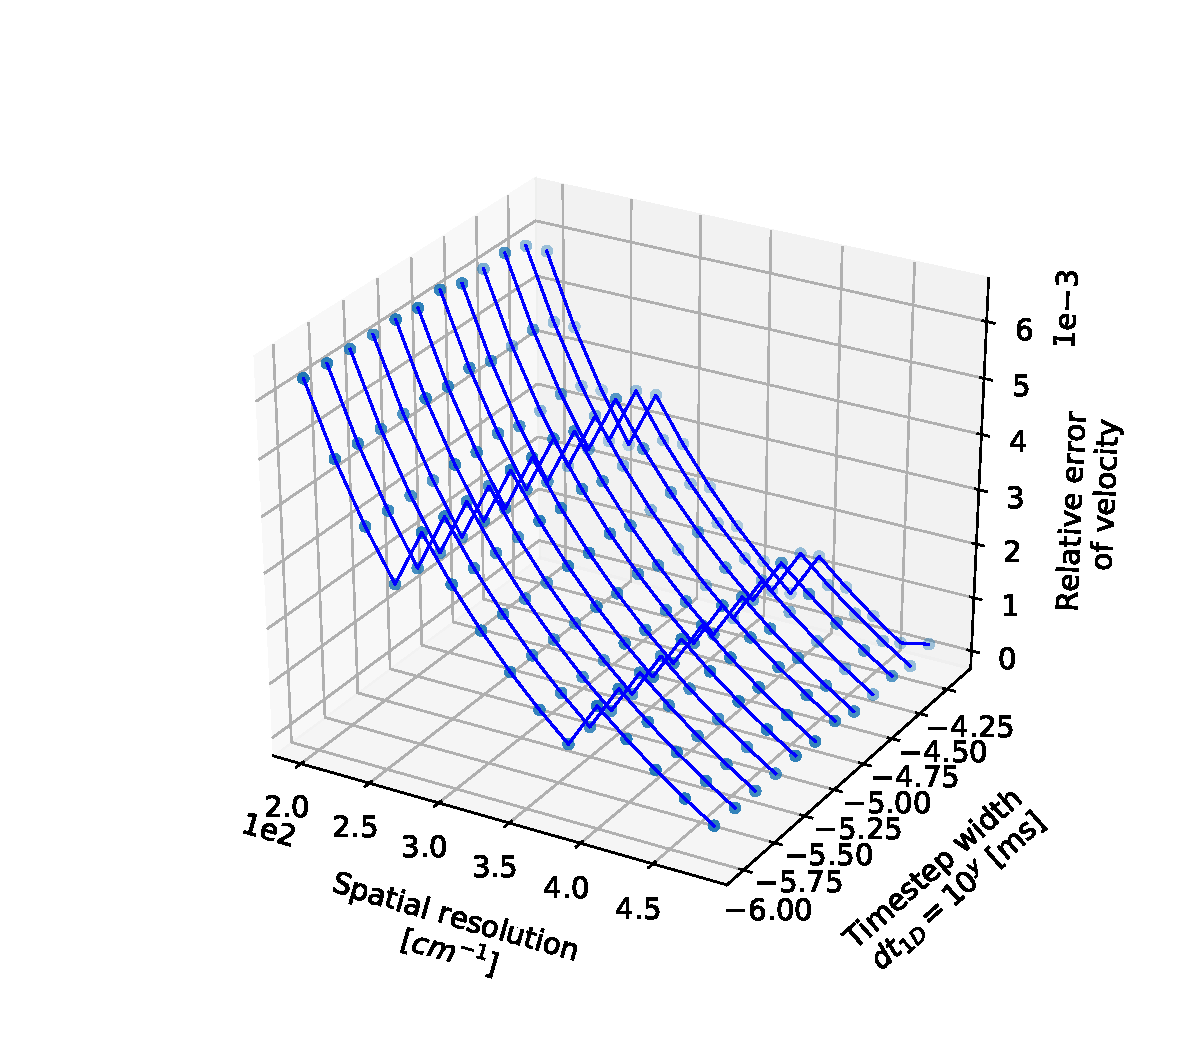
\includegraphics[width=0.8\textwidth]{images/results/studies/hh_cn_error_propagation_velocity_3d.pdf}%
%  \caption{Error of the action potential propagation velocity for varying mesh width and timestep width.}% 
%   \label{fig:hh_cn_error_propagation_velocity_3d}%
%\end{figure}
%Remove \cref{fig:hh_cn_error_propagation_velocity_3d} as not so clear.

\begin{reproduce_no_break}
  The scripts for this study are available in the repository at \href{https://github.com/dihu-stuttgart/performance}{github.com/dihu-stuttgart/} \href{https://github.com/dihu-stuttgart/performance}{performance} in the directory \code{opendihu/02_propagation_velocity}:
  \begin{lstlisting}[columns=fullflexible,breaklines=true,postbreak=\mbox{\textcolor{gray}{$\hookrightarrow$}\space}]
    ./run.sh
    ./plot_propagation_velocity.py
  \end{lstlisting}
\end{reproduce_no_break}

%-----
\subsection{Linear Solvers for the Multidomain Problem}\label{sec:multidomain_solvers}

% in opendihu 2021 paper
% selected multidomain solvers
\begin{figure}[H]
  \centering%
  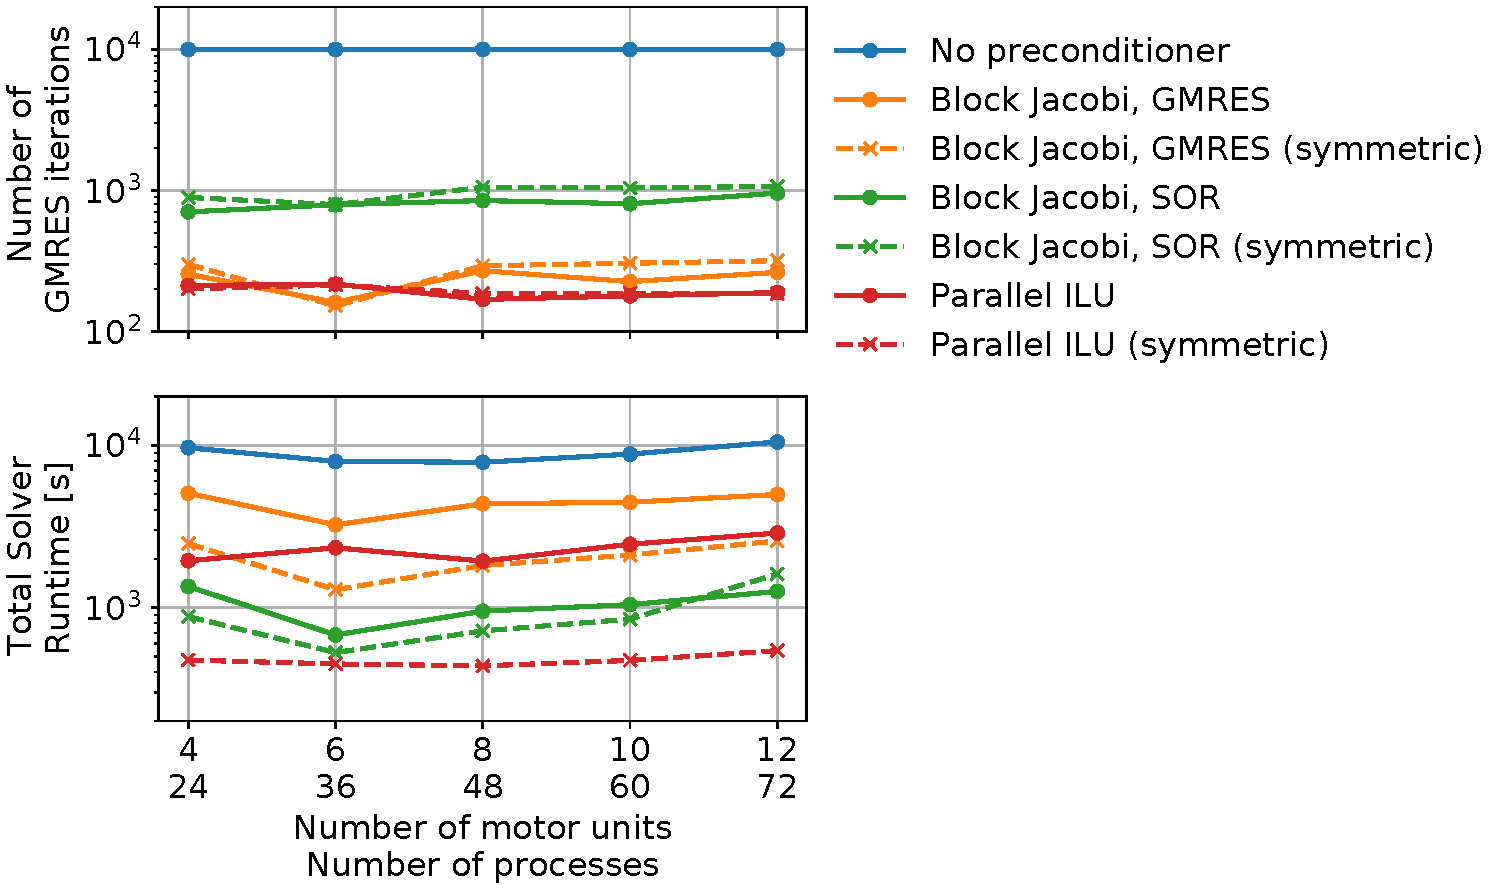
\includegraphics[width=\textwidth]{images/results/studies/multidomain_solvers_selected.pdf}%
  \caption{Evaluation of preconditioners for the multidomain model. The system is solved with a GMRES solver and different preconditioners. The upper plots shows the remaining number of iterations in the GMRES solver, the lower plot measures the total runtime of preconditioning and solution. Three different preconditioners given by orange, green and red lines are compared to the blue reference curve of using no preconditioner.}%
  \label{fig:multidomain_solver}%
\end{figure}

In the next study, we investigate the parallel weak scaling behavior for the multidomain model
with a particular focus on the total runtimes for different choices of the preconditioner that is used in the solution of the linear system of equations. Our goal is to select the fastest solver-preconditioner combination to speed up the computation of the multidomain model.

In contrast to classical weak scaling, we increase the number of MUs with the number of processes, i.e., the size of the blocks in the resulting block structured matrix remains constant, whereas the number of blocks increases.

We simulate the multidomain model with a fat domain as given in \cref{sec:discretization_body_domain} and with the subcellular model of Shorten et al. \cite{Shorten2007}. 
The model is discretized by a Strang operator splitting with Heun's method for the subcellular model and an implicit Euler scheme for the multidomain equations. The timestep widths of all schemes are $\dt_\text{0D}=\dt_\text{multidomain}=\dt_\text{splitting}=\SI{5e-4}{\milli\second}$, and an end time of \SI{1e-1}{\milli\second} is used, corresponding to 200 invocations of the linear solver.

We partition the 3D computational domain, consisting of the muscle mesh with \num{50024} nodes and the fat layer mesh with \num{37000} nodes, to 24, 36, 48, 60 and 72 subdomains. In a weak scaling setup, we correspondingly simulate 4,6,8,10 and 12 MUs.
As the square-shaped system matrix contains one row of blocks for every MU plus one row of blocks for the fat mesh, the total number of rows does not scale exactly linearly with the number of MUs. In consequence, the system matrices in the five scenarios contain \num{279720}, \num{379768}, \num{479816}, \num{579864} and \num{679912} rows and columns. Thus, the problem size per process is only approximately constant in this weak scaling study.

% n dofs
% 24: 279720
% 36: 379768
% 48: 479816
% 60: 579864 
% 72: 679912

We solve the linear system of the multidomain equations by a GMRES solver, because the system matrix is non-symmetric.
The stopping threshold on the residual norm is set to \num{1e-15} and the specified maximum number of iterations is \num{1e4}. 
Different preconditioners are applied and the resulting number of GMRES iterations and the total runtime for preconditioner and solver are measured.
\Cref{fig:multidomain_solver} shows the number of GMRES iterations in the upper plot and the total runtimes in the lower plot.

For every preconditioner, the preconditioning is either performed based on the non-symmetric system matrix (solid lines) or based on a symmetric matrix that is obtained by taking all diagonal blocks of the system matrix (dashed lines), as described in \cref{sec:multidomain_diagonal_matrix}.

The reference measurement is given by the GMRES solver without any preconditioner, visualized by the blue lines in both plots.
The upper plot of \cref{fig:multidomain_solver} indicates the maximum number of \num{1e4} iterations for all measurements of the GMRES solver without preconditioner. This means that the specified tolerance of \num{1e-15} is not reached in the given number of iterations. Thus, a preconditioner is required to obtain an accurate solution.

The first examined preconditioner is the block Jacobi scheme.
A block Jacobi preconditioner divides the system matrix into blocks on the diagonal, yielding smaller problems that can each be solved individually.
The scheme is an iterative solver, which starts with an initial solution $\bfx^{(0)}$ and successively computes  approximations $\bfx^{(i+1)} = \Phi(\bfx^{(i)})$ of the solution until the residual norm reaches the specified threshold.
%The system matrix is approximated by its diagonal.

For a model problem $A\,\bfx = \bfb$, where the system matrix $A=D+L+U$ is decomposed into a matrix $D$ with blocks on the diagonal and lower and upper triangular block matrices $L$ and $U$, respectively, the preconditioning is based on the following iterative computation scheme $\Phi: \bfx^{(i)} \mapsto \bfx^{(i+1)}$:
\begin{align}\label{eq:jacobi_iteration}
  D\,\bfx^{(i+1)} = \bfb - (L+U)\bfx^{(i)}.
\end{align}
Because of the structure of the block diagonal matrix $D$, the system is decoupled and every process can solve its own linear system of equations using the respective diagonal block as system matrix. If the symmetric option for the system matrix used in the preconditioner is chosen, the matrices $L$ and $U$ vanish and the solution of \cref{eq:jacobi_iteration} is trivial.

The preconditioner is constructed using the reordered matrix layout described in \cref{sec:structure_multidomain_system_matrix} and the symmetric matrix is obtained as discussed in \cref{sec:multidomain_diagonal_matrix}. The remaining blocks on the matrix diagonal belong to the subdomains of the parallel partitioning. Each block corresponds to a part of the mesh for all MU compartments.

Two versions of block Jacobi preconditioners provided by the PETSc library are evaluated.
The first variant, shown by the orange lines in \cref{fig:multidomain_solver}, employs a GMRES solver for the resulting smaller linear systems of equations in \cref{eq:jacobi_iteration}.
The second variant, shown by the green lines in \cref{fig:multidomain_solver}, uses a SOR (successive over-relaxation) solver with over-relaxation parameter 
$\omega=1$, i.e., a Gauß-Seidel scheme.

The upper plot in \cref{fig:multidomain_solver} shows that the number of GMRES solver iterations is reduced more for the GMRES solver than for the Gauß-Seidel solver, as the constant number of GMRES iterations in the preconditioner yields a better approximation to the solution than the same number of Gauß-Seidel iterations. The lower plot shows a smaller total runtime for the block Jacobi scheme with Gauß-Seidel solver than for the block Jacobi scheme with GMRES solver. This means that the lower runtime of the Gauß-Seidel solver in the preconditioner outweighs the larger number of GMRES iterations in the solver, compared to the GMRES preconditioning scheme. For both preconditioners, the total runtime for the variant with the symmetric matrix is lower than for the variant with the full system matrix.

Another solver is \emph{Euclid} \cite{euclid} from the HYPRE package, shown by the red lines in \cref{fig:multidomain_solver}. It is a parallel implementation of incomplete LU factorization using graph partitioning and a two-level ordering strategy.

The plots in \cref{fig:multidomain_solver} show a low number of remaining GMRES iterations after the preconditioner has been applied, similar to the block Jacobi scheme with GMRES solver. However, the total runtime of Euclid is significantly lower than the runtime of the GMRES-block Jacobi scheme. If the symmetric system matrix is used for preconditioning, the total runtime is the lowest of all measured preconditioner combinations.

Regarding the parallel weak scaling, the lower plot in \cref{fig:multidomain_solver} shows overall good scaling properties for all considered preconditioners. The runtimes slightly decrease from the first to the second data points, as the system matrix size per process also slightly decreases. Then, a trend of slightly increasing runtimes in the weak scaling setup can be seen, which indicates that the preconditioners and the GMRES solver perform slightly more computations and communication for larger problem sizes. The accuracy of the preconditioning step is not affected by the overall problem size, as can be seen by the constant numbers of GMRES iterations in the upper plot of \cref{fig:multidomain_solver}.

As a result, we use the combination of Euclid preconditioner and GMRES solver in all solutions of the multidomain model in this work, because this is the fastest of the tested combinations. Apart from the three presented preconditioners, more available choices in the software packages PETSc and HYPRE were tested, but yielded worse performance. These include the \emph{Parallel Incomplete Factorization preconditioner} (PILUT) from the HYPRE package and the combinations of the block Jacobi scheme with an algebraic multigrid method or the Euclid preconditioner for the subproblems. Tests with the parallel algebraic multigrid method \emph{BoomerAMG} from the HYPRE package also showed promising results with even lower total runtimes than the Euclid preconditioner, but suffered from occasional long runtimes and divergence in a non-deterministic fashion. However, the full set of possible parameters such as different coarsening and interpolation options and settings for the smoother have not yet been evaluated and, after fine-tuning, corresponding performance improvements could be possible in future work.

\begin{reproduce_no_break}
  The script for this study is available in the repository at \href{https://github.com/dihu-stuttgart/performance}{github.com/dihu-stuttgart/} \href{https://github.com/dihu-stuttgart/performance}{performance} in the directory \code{opendihu/07_multidomain_solver}:
  \begin{lstlisting}[columns=fullflexible,breaklines=true,postbreak=\mbox{\textcolor{gray}{$\hookrightarrow$}\space}]
    ./run_mu.sh
  \end{lstlisting}
\end{reproduce_no_break}

% scenarioName                                                                 nRanks                                                                                                              
% gmres_bjacobi_dt0.0005_atol1e-15_rtol1e-15_theta1.0_symFalse_lumpFalse_10mus 60      [6, 1, 10]   4444.074833   4472.546500  13.081118   4458.698333     -28.471667    0.0    226.0  0.997 GB  60
% gmres_bjacobi_dt0.0005_atol1e-15_rtol1e-15_theta1.0_symFalse_lumpFalse_12mus 72      [6, 1, 12]   4953.106806   4992.944583  14.215069   4977.854306     -39.837778    0.0    263.0  1.026 GB  72
% gmres_bjacobi_dt0.0005_atol1e-15_rtol1e-15_theta1.0_symFalse_lumpFalse_4mus  24       [4, 1, 6]   5050.243750   5081.276667  11.882062   5068.834583     -31.032917    0.0    255.0  1.389 GB  24
% gmres_bjacobi_dt0.0005_atol1e-15_rtol1e-15_theta1.0_symFalse_lumpFalse_6mus  36       [4, 1, 9]   3234.057500   3248.998333  12.351108   3235.983889     -14.940833    0.0    161.0  0.841 GB  36
% gmres_bjacobi_dt0.0005_atol1e-15_rtol1e-15_theta1.0_symFalse_lumpFalse_8mus  48       [6, 1, 8]   4328.314167   4374.314375  12.322344   4361.300417     -46.000208    0.0    270.0  1.087 GB  48
% gmres_bjacobi_dt0.0005_atol1e-15_rtol1e-15_theta1.0_symTrue_lumpFalse_10mus  60      [6, 1, 10]   2088.741667   2122.034500  13.006847   2108.233667     -33.292833    0.0    305.0  1.074 GB  60
% gmres_bjacobi_dt0.0005_atol1e-15_rtol1e-15_theta1.0_symTrue_lumpFalse_12mus  72      [6, 1, 12]   2549.413056   2589.060139  14.305833   2573.819167     -39.647083    0.0    318.0  1.120 GB  72
% gmres_bjacobi_dt0.0005_atol1e-15_rtol1e-15_theta1.0_symTrue_lumpFalse_4mus   24       [4, 1, 6]   2478.502500   2493.367083  11.744517   2481.051667     -14.864583    0.0    300.0  1.542 GB  24
% gmres_bjacobi_dt0.0005_atol1e-15_rtol1e-15_theta1.0_symTrue_lumpFalse_6mus   36       [4, 1, 9]   1299.019722   1301.245000  12.244350   1288.295833      -2.225278    0.0    152.0  0.827 GB  36
% gmres_bjacobi_dt0.0005_atol1e-15_rtol1e-15_theta1.0_symTrue_lumpFalse_8mus   48       [6, 1, 8]   1801.928542   1830.392917  12.377065   1817.272500     -28.464375    0.0    293.0  1.069 GB  48
% gmres_euclid_dt0.0005_atol1e-15_rtol1e-15_theta1.0_symFalse_lumpFalse_10mus  60      [6, 1, 10]   2489.941833   2471.670167  13.204272   2457.642167      18.271667    0.0    179.0  0.510 GB  60
% gmres_euclid_dt0.0005_atol1e-15_rtol1e-15_theta1.0_symFalse_lumpFalse_12mus  72      [6, 1, 12]   2914.482639   2895.433472  14.660654   2879.770000      19.049167    0.0    189.0  0.551 GB  72
% gmres_euclid_dt0.0005_atol1e-15_rtol1e-15_theta1.0_symFalse_lumpFalse_4mus   24       [4, 1, 6]   1974.359167   1954.868333  11.758821   1942.513750      19.490833    0.0    212.0  0.473 GB  24
% gmres_euclid_dt0.0005_atol1e-15_rtol1e-15_theta1.0_symFalse_lumpFalse_6mus   36       [4, 1, 9]   2366.323333   2349.646111  12.330914   2336.598333      16.677222    0.0    217.0  0.437 GB  36
% gmres_euclid_dt0.0005_atol1e-15_rtol1e-15_theta1.0_symFalse_lumpFalse_8mus   48       [6, 1, 8]   1963.516458   1945.901875  12.508950   1932.620625      17.614583    0.0    169.0  0.471 GB  48
% gmres_euclid_dt0.0005_atol1e-15_rtol1e-15_theta1.0_symTrue_lumpFalse_10mus   60      [6, 1, 10]    506.561333    486.702183  13.177800    472.658200      19.859150    0.0    187.0  0.470 GB  60
% gmres_euclid_dt0.0005_atol1e-15_rtol1e-15_theta1.0_symTrue_lumpFalse_12mus   72      [6, 1, 12]    577.824583    558.374014  14.584994    542.841681      19.450569    0.0    185.0  0.518 GB  72
% gmres_euclid_dt0.0005_atol1e-15_rtol1e-15_theta1.0_symTrue_lumpFalse_4mus    24       [4, 1, 6]    509.154167    487.713333  11.844267    475.261125      21.440833    0.0    201.0  0.448 GB  24
% gmres_euclid_dt0.0005_atol1e-15_rtol1e-15_theta1.0_symTrue_lumpFalse_6mus    36       [4, 1, 9]    480.553056    462.281917  12.279769    449.267556      18.271139    0.0    214.0  0.409 GB  36
% gmres_euclid_dt0.0005_atol1e-15_rtol1e-15_theta1.0_symTrue_lumpFalse_8mus    48       [6, 1, 8]    469.558750    450.701521  12.482108    437.435708      18.857229    0.0    186.0  0.433 GB  48
% gmres_none_dt0.0005_atol1e-15_rtol1e-15_theta1.0_symFalse_lumpFalse_10mus    60      [6, 1, 10]   8697.286500   8841.893667  14.195788   8826.917167    -144.607167    0.0  10000.0  2.184 GB  60
% gmres_none_dt0.0005_atol1e-15_rtol1e-15_theta1.0_symFalse_lumpFalse_12mus    72      [6, 1, 12]  10342.686111  10501.216667  15.572006  10484.729167    -158.530556    0.0  10000.0  2.536 GB  72
% gmres_none_dt0.0005_atol1e-15_rtol1e-15_theta1.0_symFalse_lumpFalse_4mus     24       [4, 1, 6]   9229.770417   9675.692083  14.665854   9660.403333    -445.921667    0.0  10000.0  2.006 GB  24
% gmres_none_dt0.0005_atol1e-15_rtol1e-15_theta1.0_symFalse_lumpFalse_6mus     36       [4, 1, 9]   7886.560833   7975.463611  13.603492   7961.178056     -88.902778    0.0  10000.0  1.982 GB  36
% gmres_none_dt0.0005_atol1e-15_rtol1e-15_theta1.0_symFalse_lumpFalse_8mus     48       [6, 1, 8]   7728.828542   7876.260625  13.214875   7862.334583    -147.432083    0.0  10000.0  2.145 GB  48
% gmres_sor_dt0.0005_atol1e-15_rtol1e-15_theta1.0_symFalse_lumpFalse_10mus     60      [6, 1, 10]   1064.128667   1056.613667  13.017858   1042.770333       7.515000    0.0    805.0  0.514 GB  60
% gmres_sor_dt0.0005_atol1e-15_rtol1e-15_theta1.0_symFalse_lumpFalse_12mus     72      [6, 1, 12]   1282.427083   1274.231389  14.543176   1258.699861       8.195694    0.0    959.0  0.572 GB  72
% gmres_sor_dt0.0005_atol1e-15_rtol1e-15_theta1.0_symFalse_lumpFalse_4mus      24       [4, 1, 6]   1314.639167   1366.876250  15.078050   1351.132917     -52.237083    0.0    705.0  0.470 GB  24
% gmres_sor_dt0.0005_atol1e-15_rtol1e-15_theta1.0_symFalse_lumpFalse_6mus      36       [4, 1, 9]    703.937778    691.388333  12.411444    678.247556      12.549444    0.0    793.0  0.433 GB  36
% gmres_sor_dt0.0005_atol1e-15_rtol1e-15_theta1.0_symFalse_lumpFalse_8mus      48       [6, 1, 8]    972.381875    963.809000  12.346906    950.696875       8.572875    0.0    849.0  0.511 GB  48
% gmres_sor_dt0.0005_atol1e-15_rtol1e-15_theta1.0_symTrue_lumpFalse_10mus      60      [6, 1, 10]    869.906333    862.904083  13.149073    848.941350       7.002250    0.0   1042.0  0.553 GB  60
% gmres_sor_dt0.0005_atol1e-15_rtol1e-15_theta1.0_symTrue_lumpFalse_12mus      72      [6, 1, 12]   1606.299028   1628.942917  17.998925   1609.921528     -22.643889    0.0   1070.0  0.575 GB  72
% gmres_sor_dt0.0005_atol1e-15_rtol1e-15_theta1.0_symTrue_lumpFalse_4mus       24       [4, 1, 6]    917.225833    896.343042  14.958108    880.731083      20.882792    0.0    893.0  0.495 GB  24
% gmres_sor_dt0.0005_atol1e-15_rtol1e-15_theta1.0_symTrue_lumpFalse_6mus       36       [4, 1, 9]    552.407222    540.981389  12.264922    527.989472      11.425833    0.0    794.0  0.452 GB  36
% gmres_sor_dt0.0005_atol1e-15_rtol1e-15_theta1.0_symTrue_lumpFalse_8mus       48       [6, 1, 8]    739.617708    732.262771  12.567985    718.927312       7.354937    0.0   1055.0  0.526 GB  48


% ==============
%
% --------------
%-----
%\section{Parallel in Time master thesis}
%maybe
%-----
%-----
%\section{Output file sizes}
%no
%-----
%\section{Mesh convergence, stochastic with different MU assignments}
%-----
%\section{dx-dt dependencies} 
%no
%-----
%\section{Load balancing bachelor thesis}
%no
%-----
%\section{Application of opendihu within the field of robotics} 
%no

% ------------
%
% f===========

